% This file was converted to LaTeX by Writer2LaTeX ver. 1.0.2
% see http://writer2latex.sourceforge.net for more info
\documentclass[twoside,letterpaper]{article}
\usepackage[latin1]{inputenc}
\usepackage[T1]{fontenc}
\usepackage[english]{babel}
\usepackage{amsmath}
\usepackage{amssymb,amsfonts,textcomp}
\usepackage{color}
\usepackage{array}
\usepackage{lscape}
\usepackage{supertabular}
\usepackage{hhline}
\usepackage{hyperref}
\usepackage{multirow}
\hypersetup{pdftex, colorlinks=true, linkcolor=blue, citecolor=blue, filecolor=blue, urlcolor=blue, pdftitle=SYSTEM AND SOFTWARE ARCHITECTURAL AND DETAILED DESIGN DESCRIPTI, pdfauthor=Clinton Jeffery, pdfsubject=, pdfkeywords=}
\usepackage[pdftex]{graphicx}
% Outline numbering
\setcounter{secnumdepth}{5}
\renewcommand\thesection{\arabic{section}}
\renewcommand\thesubsection{\arabic{section}.\arabic{subsection}}
\renewcommand\thesubsubsection{\arabic{section}.\arabic{subsection}.\arabic{subsubsection}}
\renewcommand\theparagraph{\arabic{section}.\arabic{subsection}.\arabic{subsubsection}.\arabic{paragraph}}
\renewcommand\thesubparagraph{\arabic{section}.\arabic{subsection}.\arabic{subsubsection}.\arabic{paragraph}.\arabic{subparagraph}}
\makeatletter
\newcommand\arraybslash{\let\\\@arraycr}
\makeatother
% List styles
\newcommand\liststyleWWviiiNumii{%
\renewcommand\theenumi{\arabic{enumi}}
\renewcommand\theenumii{\arabic{enumii}}
\renewcommand\theenumiii{\arabic{enumiii}}
\renewcommand\theenumiv{\arabic{enumiv}}
\renewcommand\labelenumi{\theenumi)}
\renewcommand\labelenumii{\theenumii.}
\renewcommand\labelenumiii{\theenumiii.}
\renewcommand\labelenumiv{\theenumiv.}
}
% Page layout (geometry)
\setlength\voffset{-1in}
\setlength\hoffset{-1in}
\setlength\topmargin{0.5in}
\setlength\oddsidemargin{1in}
\setlength\evensidemargin{1in}
\setlength\textheight{8.278in}
\setlength\textwidth{6.5in}
\setlength\footskip{0.561in}
\setlength\headheight{0.5in}
\setlength\headsep{0.461in}
% Footnote rule
\setlength{\skip\footins}{0.0469in}
\renewcommand\footnoterule{\vspace*{-0.0071in}\setlength\leftskip{0pt}\setlength\rightskip{0pt plus 1fil}\noindent\textcolor{black}{\rule{0.25\columnwidth}{0.0071in}}\vspace*{0.0398in}}
% Pages styles
\makeatletter
\newcommand\ps@Standard{
  \renewcommand\@oddhead{}
  \renewcommand\@evenhead{\@oddhead}
  \renewcommand\@oddfoot{{\textcolor{black}{\hfill SSDD Page }}{\textcolor{black}{\thepage{}}}}
  \renewcommand\@evenfoot{\@oddfoot}
  \renewcommand\thepage{\arabic{page}}
}
\newcommand\ps@Convertix{
  \renewcommand\@oddhead{}
  \renewcommand\@evenhead{\@oddhead}
  \renewcommand\@oddfoot{}
  \renewcommand\@evenfoot{\@oddfoot}
  \renewcommand\thepage{\arabic{page}}
}
\newcommand\ps@Convertviii{
  \renewcommand\@oddhead{}
  \renewcommand\@evenhead{\@oddhead}
  \renewcommand\@oddfoot{}
  \renewcommand\@evenfoot{\@oddfoot}
  \renewcommand\thepage{\arabic{page}}
}
\newcommand\ps@Convertvii{
  \renewcommand\@oddhead{}
  \renewcommand\@evenhead{\@oddhead}
  \renewcommand\@oddfoot{}
  \renewcommand\@evenfoot{\@oddfoot}
  \renewcommand\thepage{\arabic{page}}
}
\newcommand\ps@Convertvi{
  \renewcommand\@oddhead{}
  \renewcommand\@evenhead{\@oddhead}
  \renewcommand\@oddfoot{}
  \renewcommand\@evenfoot{\@oddfoot}
  \renewcommand\thepage{\arabic{page}}
}
\newcommand\ps@Convertiv{
  \renewcommand\@oddhead{}
  \renewcommand\@evenhead{\@oddhead}
  \renewcommand\@oddfoot{}
  \renewcommand\@evenfoot{\@oddfoot}
  \renewcommand\thepage{\arabic{page}}
}
\newcommand\ps@FirstPage{
  \renewcommand\@oddhead{}
  \renewcommand\@evenhead{\@oddhead}
  \renewcommand\@oddfoot{{\textcolor{black}{\hfill SSDD Page }}
{\textcolor{black}{\thepage{}}}}
  \renewcommand\@evenfoot{\@oddfoot}
  \renewcommand\thepage{\arabic{page}}
}
\makeatother
\pagestyle{Standard}
\setlength\tabcolsep{1mm}
\renewcommand\arraystretch{1.3}
\title{SYSTEM AND SOFTWARE ARCHITECTURAL AND DETAILED DESIGN DESCRIPTI}
\author{Clinton Jeffery}
\date{2010-11-18T11:30:10.24}
\begin{document}


\clearpage

{\centering\selectlanguage{english}\bfseries\color{black}
SYSTEM AND SOFTWARE DESIGN DESCRIPTION (SSDD): Incorporating
Architectural Views and Detailed Design Criteria
\par}

{\centering\selectlanguage{english}\bfseries\color{black}
FOR
\par}

\bigskip

{\centering\selectlanguage{english}\bfseries\color{black}
Phunctional UML Editor
\\(pUML)
\par}


\bigskip


\bigskip


\bigskip

\begin{figure}
\centering

\includegraphics[width=3.5in]{uidahologo.jpg}
\end{figure}

\bigskip

\bigskip

{\centering\bfseries Version 1.0 
\par}

{\centering\bfseries May 10, 2012 
\par}

\bigskip


\bigskip

{\centering\bfseries Prepared for: 
\par}

{\centering\bfseries Dr. Clint Jeffery
\par}

\bigskip


\bigskip

{\centering\bfseries Prepared by:
\par}

{\centering\bfseries
  Josh Armstrong
\\Zach Curtis
\\Brian Bowles
\\Logan Evans
\\Jeremy Klas
\\Nathan Krussel
\\Maxine Major
\\Morgan Weir
\\David Wells
\par}

{\centering\bfseries University of Idaho \par}

{\centering\bfseries Moscow, ID \ 83844-1010 \par}




\clearpage{\centering\selectlanguage{english}\bfseries\color{black}
CS383 SSDD
\par}


{\centering\selectlanguage{english}\bfseries\color{black}
RECORD OF CHANGES (Change History)
\par}



\begin{flushleft}
\tablehead{}
\begin{supertabular}[c]{|m{0.75in}|m{1.0in}|m{1.5in}|m{0.25in}|m{2in}|c|}
\hline

\centering \bfseries Change
\centering \bfseries Number
&

\centering \bfseries Date
\par
&

\centering \bfseries Location of change\newline
\centering \bfseries(e.g., page or figure \#)
&

\centering \bfseries A\newline
\centering \bfseries M\newline
\centering \bfseries D  
&

\centering \bfseries Brief description\newline
\centering \bfseries of change
&
\bfseries Initials

\\\hline
\centering 1
& 01/17/2012
& SSDD
& \centering A
& Added updated SSRS/SSDD pdf and TeX files
& MM

\\\hline
\centering 2
& 02/01/2012
& SSDD 
& \centering A
& Updated SSRS and SSDD
& MM

\\\hline
\centering 3
& 02/13/2012
& Section 4.1
& \centering M
& Class diagram reflects node factory addition
& MM

\\\hline
\centering 4
& 05/08/2012
& SSDD
& \centering M
& Document overhaul including sections, references, and class diagrams
& MM

\\\hline
\centering 5
& 05/10/2012
& SSDD
& \centering M
& Interaction diagrams section overhaul
& MM

\\\hline
\end{supertabular}
\end{flushleft}


{\selectlanguage{english}\color{black}
A - ADDED \ M - MODIFIED \ D -- DELETED}

\clearpage{\centering\selectlanguage{english}\bfseries\color{black}
Phunctional UML Editor
\par}

{\centering\selectlanguage{english}\bfseries\color{black}
TABLE OF CONTENTS
\par}

{\bfseries\color{black}
Section\ \ Page}

\setcounter{tocdepth}{3}
\renewcommand\contentsname{}
\tableofcontents

\bigskip

\bigskip

% **************************************
% SECTION 1: INTRODUCTION              *
% **************************************


\clearpage\setcounter{page}{1}\pagestyle{Convertiv}
\section[INTRODUCTION]{\bfseries\color{black}
INTRODUCTION}

\subsection{IDENTIFICATION}

{
This document is a stand-alone document and has no identification numbers other than the revision number.

\subsection[DOCUMENT PURPOSE, SCOPE, AND INTENDED AUDIENCE]
{\bfseries DOCUMENT PURPOSE, SCOPE, AND INTENDED AUDIENCE}

\subsubsection{Document Purpose}
{
Phunctional UML Editor software is being developed according to a set of requirements outlined in the pUML System and Software Requirements Specification ( Rev. 1.0 ). This document will provide detailed information regarding the design implementation of these requirements.
}

\subsubsection{Document Scope and/or Context}
{
This document includes information regarding the design and components of the pUML software. The class structure and interactions to implement features, along with rationale for these design decisions is provided.
}

\subsubsection{Intended Audience for Document}
{
This document may be referenced for educational purposes by
Computer Science students and faculty at the University of Idaho.
}

\subsection[SYSTEM AND SOFTWARE PURPOSE, SCOPE, AND INTENDED
USERS]{\bfseries SYSTEM AND
SOFTWARE PURPOSE, SCOPE, AND INTENDED USERS}


\subsubsection{System and Software Purpose}
{
The pUML software is intended to be a tool utilized by software designers to create UML diagrams. 
}

\subsubsection[System and Software Scope/or Context]{System and Software
Scope/or Context}
{
The pUML software will be designed to provide functionality to create UML diagram projects.  Users will be able to create several different types of UML diagrams, create, modify, link, save, and delete objects within individual UML diagrams, and save collections of diagrams stored as part of a project.
}

\subsubsection{Intended Users for the System and Software}
{
The completed product would be available to the general public for purchase, however this specific release will be intended strictly for use by the University of Idaho Computer Science Department students and faculty, for educational purposes only.
}


\clearpage
\subsection[DEFINITIONS, ACRONYMS, AND
ABBREVIATIONS]{\bfseries
DEFINITIONS, ACRONYMS, AND ABBREVIATIONS}

\begin{flushleft}
\tablehead{\hline
\centering \bfseries Term or
Acronym &
\centering\arraybslash \bfseries
Definition

\\\hline}
\begin{supertabular}{|m{1.3587599in}|m{5.00806in}|}
 
 AD &
 Architectural Description:
{\textquotedblleft}A collection of products to document an
architecture{\textquotedblright} ISO/IEC 42010:2007 (\S3.4).
\\\hline

 Alpha test &
 Limited release(s) to selected,
outside testers
\\\hline

 Architectural Description &
 (AD) {\textquotedblleft}A
collection of products to document an architecture{\textquotedblright}
ISO/IEC 42010:2007 (\S3.4).
\\\hline

 Architectural View &
{{\textquotedblleft}}{A
representation of a whole system from the perspective of a related set
of concerns{\textquotedblright} ISO/IEC 42010:2007 (\S3.9).}
\\\hline

 Architecture &
{{\textquotedblleft}}{The
fundamental organization of a system embodied in its components, their
relationships to each other, and to the environment, and the principles
guiding its design and evolution{\textquotedblright} ISO/IEC 42010:2007
(\S3.5).}
\\\hline

 Beta test &
 Limited release(s) to cooperating
customers wanting early access to developing systems
\\\hline

 Design Entity &
{{\textquotedblleft}}{An
element (component) of a design that is structurally and functionally
distinct from other elements and that is separately named and
referenced{\textquotedblright} IEEE STD 1016-1998 (\S3.1).}
\\\hline

 Design View &
{{\textquotedblleft}}{A
subset of design entity attribute information that is specifically
suited to the needs of a software project activity{\textquotedblright}
IEEE STD 1016-1998 (\S3.2).}\\\hline

 Final test &
 aka, Acceptance test, release of
full functionality to customer for approval\\\hline

 DFD &
 Data Flow Diagram\\\hline

 SSDD &
 System and Software Design Document\\\hline

 SSRS &
 System and Software Requirements Specification\\\hline

 System & {{\textquotedblleft}}{A
collection of components organized to accomplish a specific function or
set of functions{\textquotedblright} ISO/IEC 42010:2007
(\S3.7).}\\\hline

 System and Software Architecture and Design Description &
 An architectural and detailed design description that includes a software system within the context of its enclosing system and describes the enclosing system, the
enclosed software, and their relationship and interfaces.\\\hline

\end{supertabular}
\end{flushleft}

\bigskip

\subsection[DOCUMENT REFERENCES]
{\bfseries DOCUMENT REFERENCES}

\liststyleWWviiiNumii
\begin{enumerate}
\item {
{CSDS,
}{\textit{System and Software Requirements
Specification Template}}{, Version 1.0, July
31, 2008, Center for Secure and Dependable Systems, University of
Idaho, Moscow, ID, 83844.}}
\item {
{ISO/IEC/IEEE,
}{\textit{IEEE Std 1471-2000 Systems and
software engineering -- Recommended practice for architectural
description of software intensive systems,}}{
First edition 2007-07-15, \ International Organization for
Standardization and International Electrotechnical Commission,
(ISO/IEC), Case postale 56, CH-1211 Gen\`{e}ve 20, Switzerland, and The
Institute of Electrical and Electronics Engineers, Inc., (IEEE), 445
Hoes Lane, Piscataway, NJ 08854, USA.}}
\item {
{IEEE, }{\textit{IEEE
Std 1016-1998 Recommended Practice for Software Design
Descriptions}}{, 1998-09-23, The Institute of
Electrical and Electronics Engineers, Inc., (IEEE) 445 Hoes Lane,
Piscataway, NJ 08854, USA.}}
\item {
{3) ISO/IEC/IEEE,
}{\textit{IEEE Std. 15288-2008 Systems and
Software Engineering -- System life cycle
processes,}}{ Second edition 2008-02-01,
\ International Organization for Standardization and International
Electrotechnical Commission, (ISO/IEC), Case postale 56, CH-1211 Gen\`{e}ve
20, Switzerland, and The Institute of Electrical and Electronics
Engineers, Inc., (IEEE), 445 Hoes Lane, Piscataway, NJ 08854, USA.}}
\item {
{ISO/IEC/IEEE, IEEE Std. 12207-2008,
}{\textit{Systems and software engineering --
Software life cycle processes, }}{Second
edition 2008-02-01, \ International Organization for Standardization
and International Electrotechnical Commission, (ISO/IEC), Case postale
56, CH-1211 }{Gen\`{e}ve 20, Switzerland, and The
Institute of Electrical and Electronics Engineers, Inc., (IEEE), 445
Hoes Lane, Piscataway, NJ 08854, USA.}}
\end{enumerate}


\clearpage
\subsection{DOCUMENT OVERVIEW}

{
Section 2 of this document describes the system and software constraints
imposed by the operational environment, system requirements and user
characteristics, and then identifies the system stakeholders and lists
describes their concerns and mitigations to those concerns.}

{
Section 3 of this document describes the system and software
architecture from several viewpoints, including, but not limited to,
the developer{\textquoteright}s view and the user{\textquoteright}s
view.}

{
Section 4 provides detailed design descriptions for every component
defined in the architectural view(s). \ Sections 5 provides
traceability information connecting the original specifications
(referenced above) to the architectural components and design entities
identified in this document.}

{
Section 6 and beyond are appendices including original information and
communications used to create this document.}

\subsection[DOCUMENT
RESTRICTIONS]{\bfseries DOCUMENT
RESTRICTIONS}

{
This document is for LIMITED RELEASE ONLY to UI CS personnel working on
the project.}



% **************************************
% SECTION 2: CONSTRAINTS / STAKEHOLDER *
% **************************************

\clearpage

\section{CONSTRAINTS AND STAKEHOLDER CONCERNS}

\subsection{CONSTRAINTS}

\subsubsection{Environmental Constraints.}
{
The pUML software poses no environmental constraints at this time .
}

\subsubsection{System Requirement Constraints.}
{
The pUML software will be designed to function on, Windows 7, and Linux. Cross platform functionality will minimize portability errors and allow for projects to be migrated between platforms with minimal difficulty.  However, the pUML software is not intended to be migrated to any other platforms with any guaranteeable level of functionality. \newline
The pUML software is also not intended to be utilized by multiple users. \newline
This release will not include several features which may be industry standard for UML diagram editors. These features would be incorporated into a later software release.
}

\subsubsection{User Characteristic Constraints.}
{
University of Idaho Computer Science students and faculty should be able
to reasonably understand and operate the pUML software.
}

\subsection[STAKEHOLDER CONCERNS]
{\bfseries STAKEHOLDER CONCERNS}
{
There are no stakeholders for our software at this time.
}


\bigskip


% *********************************************
% SECTION 3: SYSTEM AND SOFTWARE ARCHITECTURE *
% *********************************************


\clearpage\setcounter{page}{1}\pagestyle{Convertvi}
\section[SYSTEM AND SOFTWARE
ARCHITECTURE]{\bfseries SYSTEM AND
SOFTWARE ARCHITECTURE}

\subsection[DEVELOPER{\textquoteright}S ARCHITECTURAL
VIEW]{\bfseries
DEVELOPER{\textquoteright}S ARCHITECTURAL VIEW}

\subsubsection[Developer{\textquoteright}s View
Identification]{\bfseries
Developer{\textquoteright}s View Identification}
{
This is the architecture of the program from the viewpoint of the
developer. The purpose is to give an overview of the details of the major
components of the architecture.}

{
In order to have the program be able to draw diagrams, a custom QWidget
is defined called the Canvas. The Canvas holds all the instantiations of
nodes and draws each one. It also creates the nodes by handling the
mouse click events. The toolbar and menu system lets the Canvas know
which type of object will be created next. The Canvas is a member of
the MainWindow class, which inherits from QMainWindow. }

\subsubsection[Developer{\textquoteright}s View Representation and
Description ]{Developer{\textquoteright}s View Representation and
Description }

{
The Canvas contains a vector container of
ObjectNodes. Each ObjectNode has a draw function which takes a QPainter
reference as an argument and draws the appropriate figure with the
QPainter. The program then defines it's own ObjectNodes, e.g. CircleNode
and DiamondNode, and pushes them into the vector. In this way the Canvas
can draw each of the nodes in the diagram. To create a new object, it
handles a mouse click event and creates a new object of the type specified
by a previous call to it's function to set a new object type. The new
object is pushed into the vector and then the draw function is called
on every node in that vector. When selecting a node to edit or delete,
the Canvas takes the X and Y coordinates of the click and translates that
into the index of the object selected. Then the Canvas can popup a menu
to edit the node or delete the node. }


\subsubsection{Developer{\textquoteright}s Architectural Rationale}

{
We decided to create a new QWidget for the Canvas so that it can handle
click events and have a paint function. We then decided to have the nodes
represented by a vector so that it can be easily iterated over and quickly
accessed by index. We decided to have the nodes be represented by specific
definitions of ObjectNodes so that they can all be pushed into the a vector
ObjectNodes. This way each of the nodes can define their own draw function,
as well private data such as radius for circles. This allows new objects to
be easily created. }

\clearpage
\subsection[USER{\textquoteright}S ARCHITECTURAL VIEW]
{\bfseries USER{\textquoteright}S ARCHITECTURAL VIEW}

\subsubsection{User{\textquoteright}s View Identification}
{
This is the viewpoint of the program from the viewpoint of the user.
From this viewpoint, there are three major components of the
program: the Canvas, the Toolbar and the Menu. }

\subsubsection{User{\textquoteright}s View Representation and
Description }
{
The menu and the toolbar have redundant functionality. The toolbar provides
quick access to certain menu items, such as available objects and connectors. The canvas provides a space for the user to place objects and connectors during creation of a UML diagram. The pUML software also provides options for the user to save and load pUML UML diagrams. 
}

\subsection[CONSISTENCY OF ARCHITECTURAL VIEWS]
{\bfseries CONSISTENCY OF ARCHITECTURAL VIEWS}
{
Due to the limited scope of this project, there are no known inconsistencies between views. 
}


\clearpage
\section{SOFTWARE DETAILED DESIGN}

\bigskip

\subsection[\ DEVELOPER{\textquoteright}S VIEWPOINT DETAILED SOFTWARE DESIGN]
{DEVELOPER{\textquoteright}S VIEWPOINT DETAILED SOFTWARE DESIGN }
{
Diagrams depicting classes and relationships between classes for the pUML software are provided in this section.
}

\subsubsection[\ Class Overview]
{\bfseries Class Overview}
{
This is a simplified version of the full class diagram for the pUML software.  This diagram shows the names of the main classes and the data flow between them. \newline
The nodes dependent on BaseNode are examples of node types, in this case taken from the UML Class Diagram type.  Each diagram type consists of objects and connectors, each of which are designed according to this template.
}
  \begin{figure}[h]
  \centering
  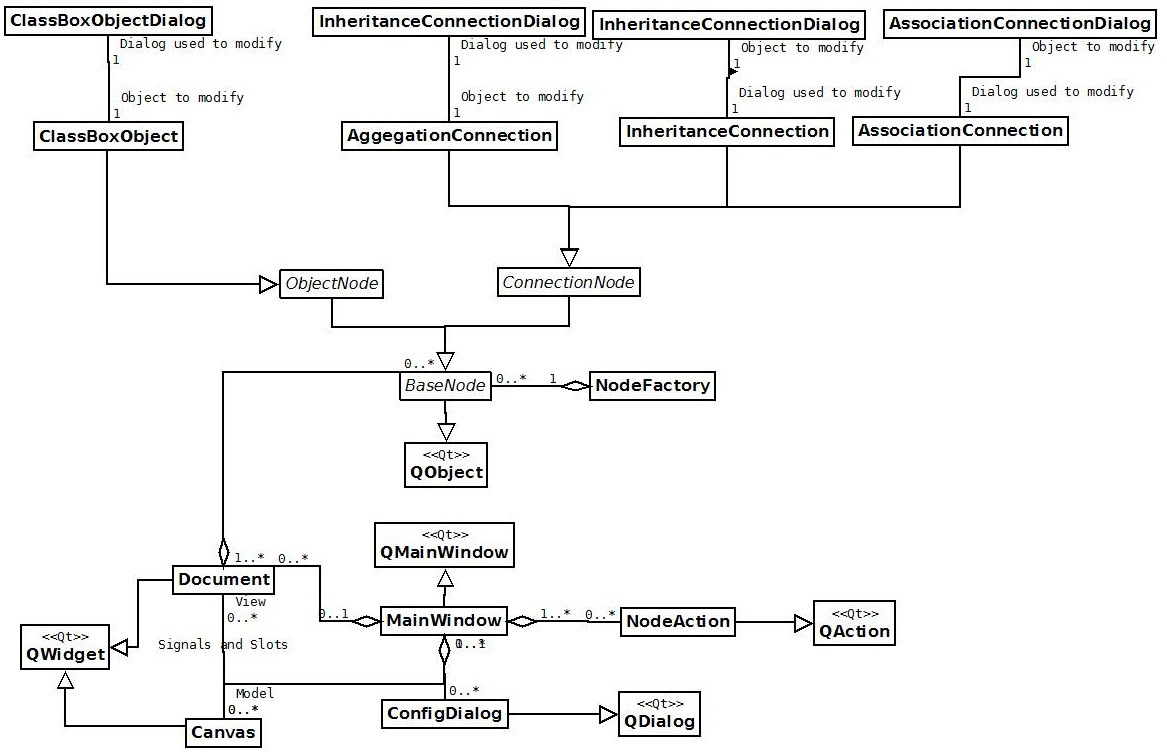
\includegraphics[width=6.5in]{class_simple.jpeg}
  \end{figure}


\clearpage
\subsubsection[\ Main Window Class ]
{\bfseries Main Window Class }
{
The MainWindow class is the controller class, joining the Document and Canvas together. This class brings together all the components of pUML at the largest scale.  This class is also responsible for guiding the process by which the various nodes appear on the canvas.
}
  \begin{figure}[h]
  \centering
  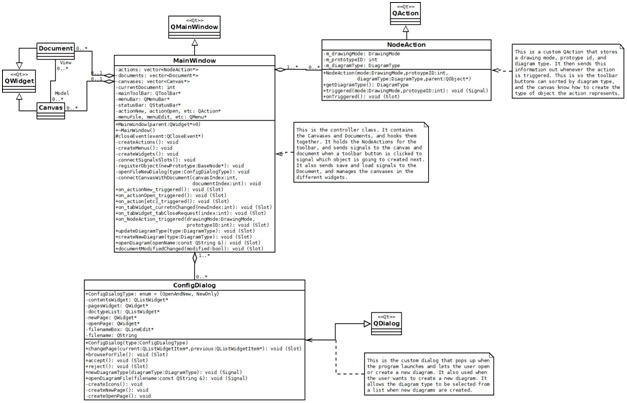
\includegraphics[width=6.5in]{class_mainwindow.jpeg}
  \end{figure}


\clearpage
\subsubsection[\ Document and Canvas Classes ]
{\bfseries Document and Canvas Classes }
{
In the Model-View system, the Document performs as the model, controlling all information about the individual nodes in a diagram, and is critical in the process of saving and loading. \newline
The Canvas class is responsible for the view, and handles all mouse events and actions related to the mouse events, including the properties dialog and node deletion.
}
  \begin{figure}[h]
  \centering
  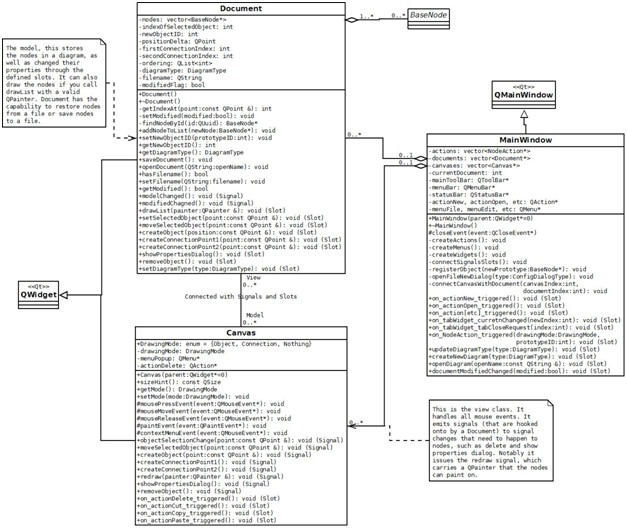
\includegraphics[width=6.5in]{class_documentcanvas.jpeg}
  \end{figure}

\clearpage
\subsubsection[\ Base Node Class ]
{\bfseries Base Node Class }
{
The BaseNode is the most abstract node class, containing all the standard information for all nodes. This class also incorporates the cloning function, which is critical in developing several copies of any type of node. \newline
The NodeFactory contains a registry of objects, and may produce copies of these objects. Together with BaseNode, each node placed on the canvas in a UML diagram is guaranteed to be purely unique, even as an exact replica of another node. 
}
  \begin{figure}[h]
  \centering
  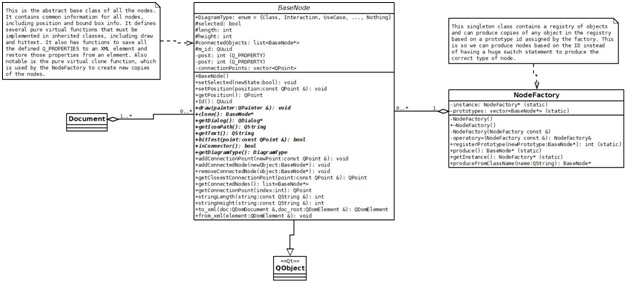
\includegraphics[width=6.5in]{class_basenode.jpeg}
  \end{figure}

\clearpage
\subsubsection[\ ConnectionNode Class ]
{\bfseries ConnnectionNode Class }
{
The ConnectionNode class incorporates both specific types of connection and the dialogs unique to each connection type. This allows for several types of connections, unique with their own dialog properties. \newline
The example shown is from a Class diagram. Connections from other diagram types would have a nearly identical format, with minor diagram-specific differences.
}
  \begin{figure}[h]
  \centering
  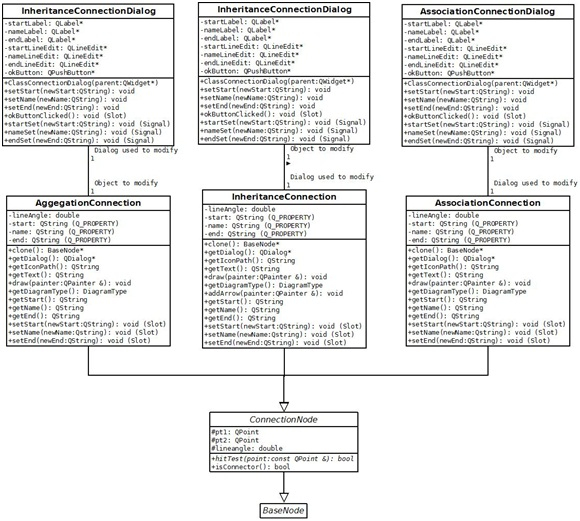
\includegraphics[width=6.5in]{class_connectionnode.jpeg}
  \end{figure}

\clearpage
\subsubsection[\ Object Node Class ]
{\bfseries Object Node Class }
{
The ObjectNode class incorporates specific object types and dialogs unique to each object type. This allows for several types of objects, unique with their own dialog properties. \newline
The example shown is from a Class diagram. Objects from other diagram types would have a nearly identical format, with minor diagram-specific differences.
}
  \begin{figure}[h]
  \centering
  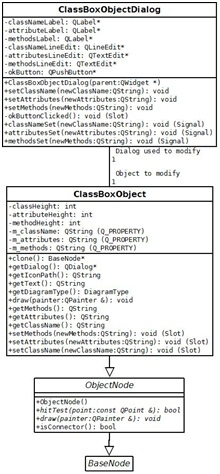
\includegraphics[width=2.5in]{class_classboxobjectnode.jpeg}
  \end{figure}




% **************************************
% COMPONENT/ENTITY DICTIONARY          *
% **************************************

\clearpage

\begin{landscape}

\subsection[COMPONENT/ENTITY DICTIONARY]
{\bfseries COMPONENT/ENTITY DICTIONARY}
{
This table shows the individual components, implemented as classes, 
utilized in the development of this software, 
and how each class is related to the other classes.
}

\begin{flushleft}
\tablehead{}
\begin{supertabular}{|m{1.65in}|m{1.0in}|m{3.0in}|m{1.65in}|m{1.65in}|}
\hline
\multicolumn{5}{|m{8.95in}|}{\centering
\bfseries Component/Entity
Dictionary}\\\hline
\centering \bfseries Name of Class &
\centering \bfseries Type/Range &
\centering \bfseries
Purpose/Function &
\centering \bfseries Dependencies &
\centering\arraybslash \bfseries
Subordinates
\\\hline

    QMainWindow 
  & QWidget \newline QMainWindow 
  & Connects the canvas and document together 
  & QMainWindow
  & ConfigDialog \newline NodeAction
\\\hline

    ConfigDialog 
  & QDialog
  & Main dialog which allows the user to select a new diagram type or open an existing diagram. 
  & MainWindow
  & N/A
\\\hline

    NodeAction 
  & QAction
  & Sets the drawing mode
  & Main Window 
  & N/A
\\\hline

    Canvas
  & QWidget
  & Draws objects and connectors 
  & Main Window 
  & N/A
\\\hline

    Document
  & QWidget 
  & Contains all diagram information
  & MainWindow 
  & N/A
\\\hline

    BaseNode
  & QObject
  & Draws the object
  & Document
  & ObjectNode \newline ConnectionNode
\\\hline

    NodeFactory
  & N/A
  & Registry of objects, which may be copied by ID
  & BaseNode
  & N/A
\\\hline

    ObjectNode
  & BaseNode
  & Contains object
  & BaseNode
  & ObjectNode \newline ConnectionNode
\\\hline

    *ObjectType
  & BaseNode
  & Contains object features
  & ObjectNode
  & *ObjectTypeDialog
\\\hline

    *ObjectTypeDialog
  & QDialog
  & Contains object dialog
  & *ObjectType
  & N/A
\\\hline

    ConnectionNode
  & BaseNode
  & Contains connection
  & BaseNode
  & *ConnectionType
\\\hline

    *ConnectionType 
  & BaseNode
  & Contains connection type
  & ConnectionNode
  & *ConnectionTypeDialog
\\\hline

    *ConnectionTypeDialog
  & QDialog
  & Contains connection features
  & *ConnectionType
  & N/A
\\\hline

\end{supertabular}
\end{flushleft}

{* Object and Connection types are varied, but follow this pattern. \newline
The names of the respective classes vary per diagram type and object/connector type, but follow the same template.
** All QT classes are not detailed in this document.
}



\end{landscape}

\clearpage

% *************************
% FEATURE DETAILED DESIGN *
% *************************

\subsection[FEATURE DETAILED DESIGN]
{\bfseries FEATURE DETAILED DESIGN}
{
Each of the diagrams in this section represent an important functionality
of the pUML software.  The interaction diagrams detail the object classes
that will be utilized in the execution of each of these major features of
the software, as well as show how these classes interact.
}


% 
% FEATURE: CREATE NEW DIAGRAM
%

\subsubsection{Detailed Design for Feature: Create New Diagram }
\paragraph[\ Introduction/Purpose of this Feature]
{\ Introduction/Purpose of this Feature}
{
Each of the UML diagrams will need its own space for development within the pUML software. The ``New'' feature allows the user to select a diagram and start developing that diagram on a blank, diagram-specific canvas.
}

\paragraph[Input for this Feature]{Input for this Feature}
{
The user selects ``New'' from the main menu options, and selects a diagram type from the Configuration Dialog box. 
}

\paragraph{Output for this Feature}
{
pUML will then load a blank canvas in a new tab, with a toolbar containing only that diagram's type of objects and connectors.
}

\paragraph{Feature Process to Convert Input to Output}
{
User selects ``New'' from main menu. MainWindow class creates a ConfigDialog box, which contains all possible diagram types. User selects diagram type. ConfigDialog returns the diagram type back to the MainWindow class, which in turn uses that information to create both the Canvas and Document classes. MainWindow then connects the Canvas and Document classes, and sends the user-selected diagram type to the Document class. The main window then creates a new tab with a blank canvas and all diagram-specific properties.
}

\paragraph{Design Constraints and Performance Requirements of this Feature}
{
 New diagrams may not be of a generic diagram type. The user must specify what type of a new diagram they will be developing prior to pUML creating the space in which to develop a UML diagram.
}
\bigskip

\begin{figure}[h]
\centering
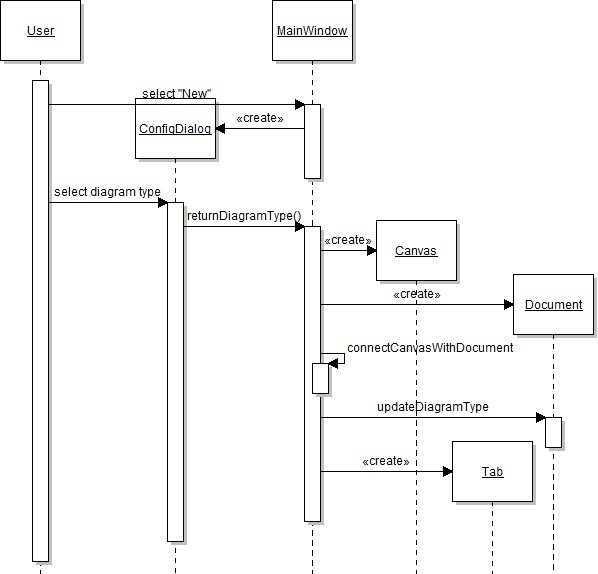
\includegraphics[width=6.0in]{IntNewDiagram.jpg}
\caption{Create New Diagram}
\end{figure}
\clearpage



% 
% FEATURE: OPEN EXISTING DIAGRAM
%

\subsubsection{Detailed Design for Feature: Open an Existing Diagram }
\paragraph[\ Introduction/Purpose of this Feature]
{\ Introduction/Purpose of this Feature}
{
The pUML software provides the Open feature so that users may store diagrams and view or edit them later.  Open will load the .puml diagram type into pUML, which will allow the user to continue modification.
}

\paragraph[Input for this Feature]{Input for this Feature}
{
User selects ``Open'' from the main menu.  The user is then prompted to locate the file on their computer.
}

\paragraph{Output for this Feature}
{
If the user-selected file is of .puml type, pUML will load the diagram into a new tab of that particular diagram type, and the diagram will be modifiable.
}

\paragraph{Feature Process to Convert Input to Output}
{
User selects ``Open'' from the MainWindow class, which creates the OpenFileDialog.  The User then selects which file they choose to open, and OpenFileDialog returns that value to MainWindow.  MainWindow creates both the Canvas and Document classes and then connects these two classes. MainWindow creates the tab for the diagram to load into, and sends diagram specific information to the Document class. The Document class then returns the diagram type to MainWindow.
}

\paragraph{Design Constraints and Performance Requirements of this Feature}
{
The pUML software will only open files of .puml type. 
}
\bigskip

\begin{figure}[h]
\centering
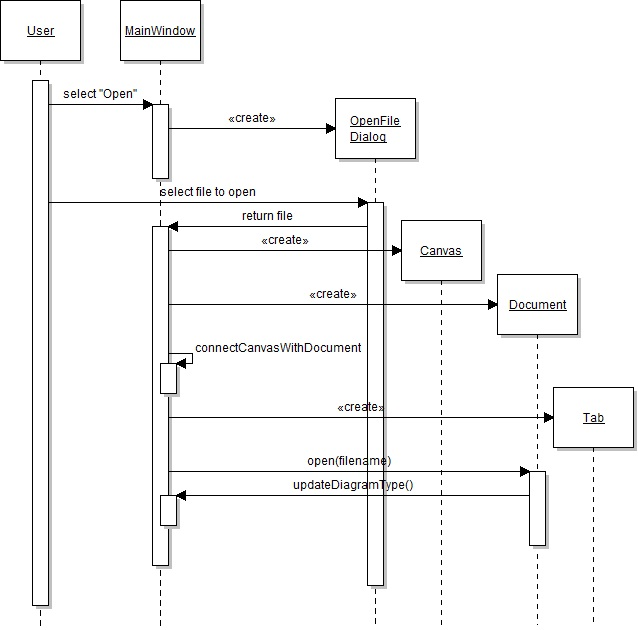
\includegraphics[width=6.0in]{IntOpen.jpg}
\caption{Open Diagram}
\end{figure}
\clearpage



% 
% FEATURE: EXIT PUML
%

\subsubsection{Detailed Design for Feature: Exit pUML }
\paragraph[\ Introduction/Purpose of this Feature]
{\ Introduction/Purpose of this Feature}
{
When the user is finished modifying UML diagrams, the pUML software may be closed.
}

\paragraph[Input for this Feature]{Input for this Feature}
{
The user clicks the ``X'' in the upper corner of the pUML main window, or selects ``Exit'' from the main menu.
}

\paragraph{Output for this Feature}
{
pUML checks to see if the file(s) being closed are saved, and once all files have been either saved or discarded, the pUML software closes.
}

\paragraph{Feature Process to Convert Input to Output}
{
User selects ``Exit'' from the main menu.  MainWindow iterates through each of the tabs and sends a request called getModified() from the Document class. As long as none of the tabs is flagged as having a modification since the previous save, then all tabs are assumed to be saved, and MainWindow closes the pUML software.
\newline
If tabs need to be saved, reference the Save feature in this document. Tabs will be saved, and this process will resume as normal from that point.
}

\paragraph{Design Constraints and Performance Requirements of this Feature}
{
pUML will also close if diagrams are not saved, and the user wishes to discard all changes. 
}
\bigskip

\begin{figure}[h]
\centering
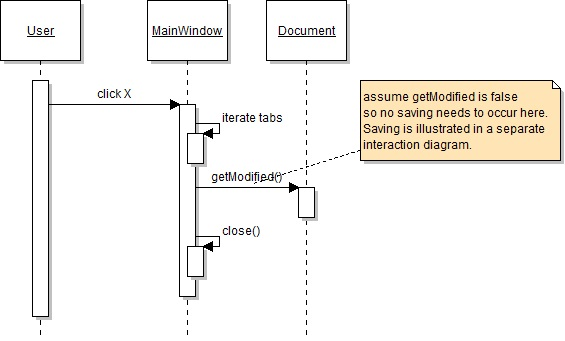
\includegraphics[width=6.0in]{IntExit.jpg}
\caption{Exit pUML}
\end{figure}
\clearpage



% 
% FEATURE: SAVE
%

\subsubsection{Detailed Design for Feature: Save }

\paragraph[\ Introduction/Purpose of this Feature]
{\ Introduction/Purpose of this Feature}
{
The user wishes to save a UML diagram.
}

\paragraph[Input for this Feature]{Input for this Feature}
{
The user opens the File Menu and selects Save.
}

\paragraph{Output for this Feature}
{
pUML checks to see if the file name that the user selects is valid, and when this is verfied, the diagram currently loaded is stored at that file location. \newline
If the file name has not previously been stored, refer to the Save As feature in this document.
}

\paragraph{Feature Process to Convert Input to Output}
{
The user clicks ``Save'' on the main menu, and MainWindow sends the current diagram name through hasFileName() to Document to verify whether or not the name has been previously stored. Document verifies that hasFileName() returns true, stores the current diagram content over the contents of the existing file, and sets modifyChanged() to hide the asterisk (indicating an unsaved diagram) at that tab.
}

\paragraph{Design Constraints and Performance Requirements of this Feature}
{
If hasFileName returns false, refer to the Save As feature in this document.
}
\bigskip
\bigskip

\begin{figure}[h]
\centering
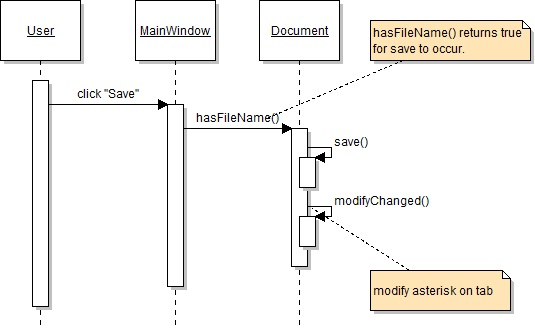
\includegraphics[width=6.0in]{IntSave.jpg}
\caption{Save Diagram}
\end{figure}

\clearpage




% 
% FEATURE: SAVE AS
%

\subsubsection{Detailed Design for Feature: Save As }

\paragraph[\ Introduction/Purpose of this Feature]
{\ Introduction/Purpose of this Feature}
{
The user wishes to save a UML diagram under a new file name.
}

\paragraph[Input for this Feature]{Input for this Feature}
{
The user selects Save As from the main menu.
}

\paragraph{Output for this Feature}
{
pUML produces a dialog box through which the user may type a new file name, and then pUML saves the file under that new name.
}

\paragraph{Feature Process to Convert Input to Output}
{
The User clicks on ``Save As'' in the main menu. \newline
Or the User attempts to save a previously unsaved file, and MainWindow sends hasFileName() to Document to verify if the current diagram name exists, which returns false. \newline
MainWindow creates a new QFileDialog into which the User enters their desired file name. The QFileDialog sends this information to MainWindow, which in turn calls setFileName() to Document, and then save().
}

\paragraph{Design Constraints and Performance Requirements of this Feature}
{
N/A
}
\bigskip
\bigskip

\begin{figure}[h]
\centering
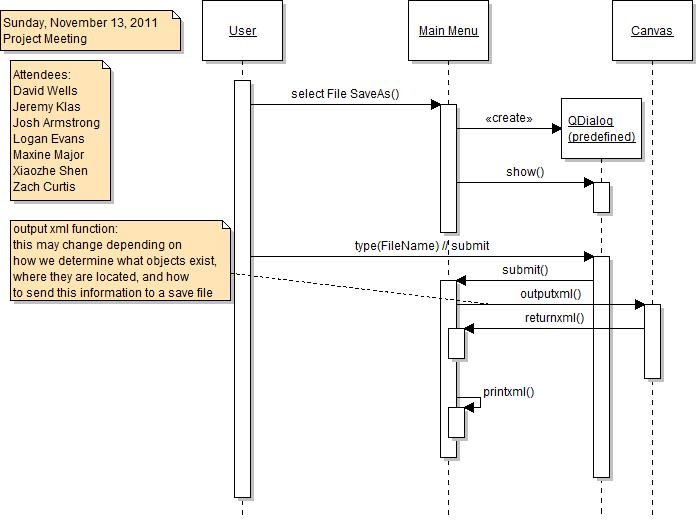
\includegraphics[width=6.0in]{IntSaveAs.jpg}
\caption{Save / Save As}
\end{figure}

\clearpage





% 
% FEATURE: CLOSE DIAGRAM TAB
%

\subsubsection{Detailed Design for Feature: Close Diagram Tab }
\paragraph[\ Introduction/Purpose of this Feature]
{\ Introduction/Purpose of this Feature}
{
The pUML software provides ability for multiple diagrams to be edited by utilizing a tabbed structure. As design complexity increases, or if the User may desire to reduce screen clutter, the ability to close tabs is very useful.
}

\paragraph[Input for this Feature]{Input for this Feature}
{
The user clicks the ``x'' on the tab.
}

\paragraph{Output for this Feature}
{
pUML checks to see if the current diagram has been saved, and when there are no outstanding modifications, the tab is closed.
}

\paragraph{Feature Process to Convert Input to Output}
{
Uesr clicks the ``x'' on the tabWidget, which uses MainWindow to send a getModified request to Document. If getModified returns false (diagram has been previously saved), then Document returns this information to MainWindow, which sends permission to the tabWidget to close itself.
}

\paragraph{Design Constraints and Performance Requirements of this Feature}
{
After all tabs in pUML have been closed, the pUML software remains open, with main menu options available. If the user is desiring to close the pUML software, then they must choose to ``Exit'' the program.
}
\bigskip

\begin{figure}[h]
\centering
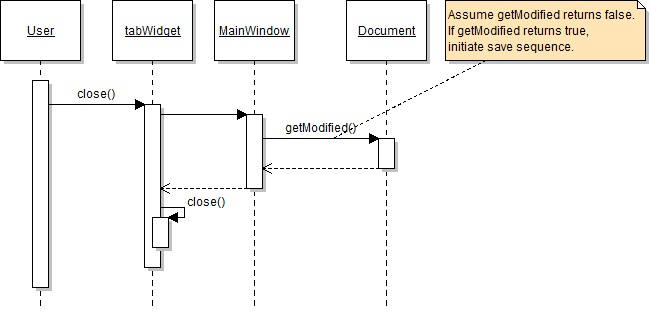
\includegraphics[width=6.0in]{IntCloseTab.jpg}
\caption{Close Diagram Tab}
\end{figure}

\clearpage


% 
% FEATURE: PLACE NEW OBJECT
%

\subsubsection{Detailed Design for Feature: Place New Object }
\paragraph[\ Introduction/Purpose of this Feature]
{\ Introduction/Purpose of this Feature}
{
The user will be able to select objects from the toolbar and place them on the Canvas.
}

\paragraph[Input for this Feature]{Input for this Feature}
{
The user will click on a shape on the toolbar.  The first subsequent click of the mouse over the Canvas area will place the selected shape at that location.
}

\paragraph{Output for this Feature}
{
The object will be placed on the Canvas, at a location of the user{\textquoteright}s choosing.
}

\paragraph{Feature Process to Convert Input to Output}
{
The mouse click on a shape on the toolbar notifies MainWindow of an objectAction(). The MainWindow sets the draw mode to object through the Canvas. The user then clicks on the canvas, which Canvas then tells Document to create the object. Document creates a new BaseNode, sends it the properties dialog, and then Document initiates showDialog().
}

\paragraph{Design Constraints and Performance Requirements of this Feature}
{
N/A
}
\bigskip
\bigskip

\begin{figure}[h]
\centering
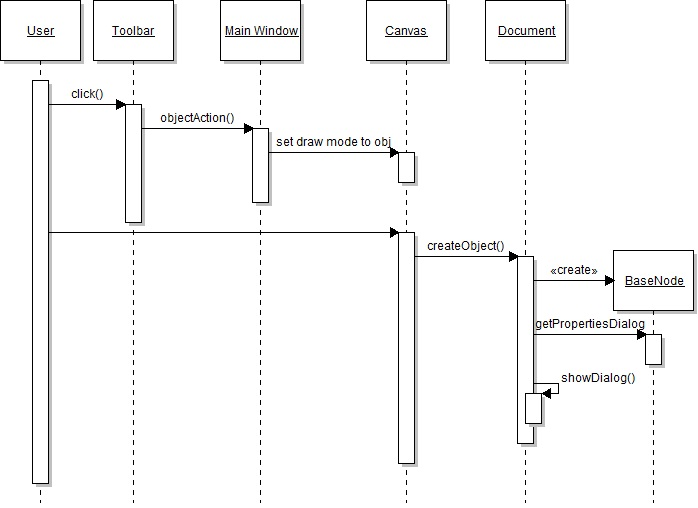
\includegraphics[width=6.0in]{IntNewObj.jpg}
\caption{Place New Object}
\end{figure}

\clearpage


% 
% FEATURE: MOVE OBJECT
%

\subsubsection{Detailed Design for Feature: Move Object }
\paragraph[\ Introduction/Purpose of this Feature]
{\ Introduction/Purpose of this Feature}
{
This gives the user the capability to rearrange objects in a UML diagram after their initial placement.
}

\paragraph[Input for this Feature]{Input for this Feature}
{
The user clicks on an object, and then drags it to another location on the canvas.
}

\paragraph{Output for this Feature}
{
The canvas displays the object at its new location.
}

\paragraph{Feature Process to Convert Input to Output}
{
The user leftclicks down on the object, on the canvas. The Canvas class tells the Document class to setSelectedObject() to true. The user moves the mouse (mouseMove event), and Canvas redraws the object at each location. Document sets the position at each move. The user releases the mouse and the Document class retains all current object location properties.
}

\paragraph{Design Constraints and Performance Requirements of this Feature}
{
Objects are permitted to overlap in pUML, which may require more diligence on the user{\textquoteright}s part.
}
\bigskip

\begin{figure}[h]
\centering
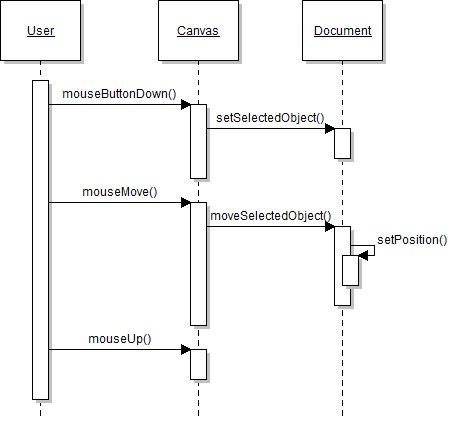
\includegraphics[width=6.0in]{IntMoveObj.jpg}
\caption{ Move Object }
\end{figure}

\clearpage




% 
% FEATURE: EDIT OBJECT DESCRIPTION
%

\subsubsection{Detailed Design for Feature: Edit Object Description}

\paragraph[\ Introduction/Purpose of this Feature]
{\ Introduction/Purpose of this Feature}
{
The user may edit an object{\textquoteright}s description.
}

\paragraph[Input for this Feature]{Input for this Feature}
{
The user right clicks on the object they wish to modify and selects ``Properties'' from the context menu.
}

\paragraph{Output for this Feature}
{
pUML displays a dialog box with object description, and after the user has submitted changes to the description, the new description is displayed on the canvas. 
}

\paragraph{Feature Process to Convert Input to Output}
{
User right clicks on an object on the Canvas. The Canvas tells Document to perform a hittest to determine whether an object resides at those coordinates. If valid, the Canvas tells Document to initiate the properties Dialog for the selected object. \newline 
The user modifies the object properties per the Dialog.  The Dialog sends the updated object information to Document.
}

\paragraph{Design Constraints and Performance Requirements of this Feature}
{
The user may only edit properties of valid objects and connectors. No other properties in pUML may be modified.
}
\bigskip
\bigskip

\begin{figure}[h]
\centering
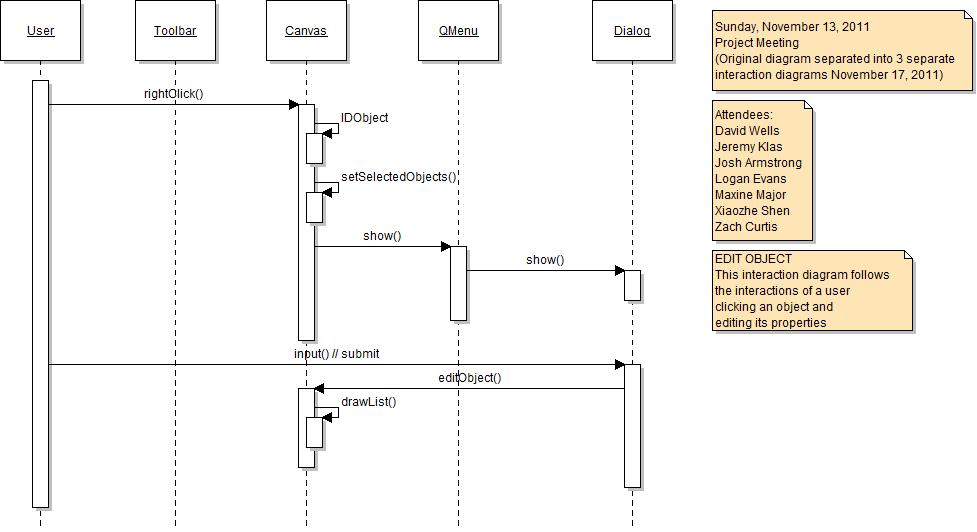
\includegraphics[width=6.0in]{IntEditObj.jpg}
\caption{Edit Object Description}
\end{figure}

\clearpage



% 
% FEATURE: DELETE OBJECT
%

\subsubsection{Detailed Design for Feature: Delete an Object}

\paragraph[\ Introduction/Purpose of this Feature]
{\ Introduction/Purpose of this Feature}
{
The user deletes an object from the Canvas.
}

\paragraph[Input for this Feature]{Input for this Feature}
{
The user right-clicks on an object to be deleted, and selects the delete option from the context menu.
}

\paragraph{Output for this Feature}
{
The object is removed from the canvas along with any connectors (connected objects).
}

\paragraph{Feature Process to Convert Input to Output}
{
User right clicks on an object on the Canvas. The Canvas verifies that an object exists at the coordinates of the click, and sets the object through Document.  The Canvas displays the context menu.  The user selects the delete option from the menu, which tells Document to delete the object and any connected objects.
}

\paragraph{Design Constraints and Performance Requirements of this Feature}
{
All connectors attached to an object will be deleted along with that object.
}
\bigskip
\bigskip

\begin{figure}[h]
\centering
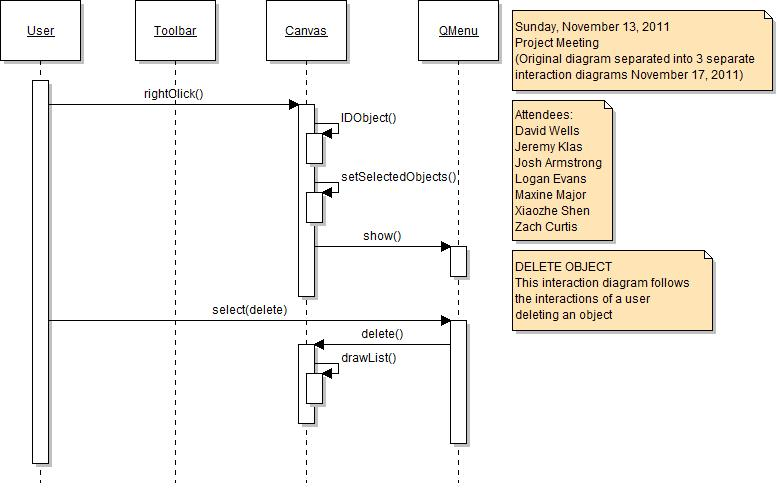
\includegraphics[width=6.0in]{IntDelObj.jpg}
\caption{Delete Object}
\end{figure}

\clearpage



% 
% FEATURE: PLACE NEW CONNECTOR
%

\subsubsection{Detailed Design for Feature: Place a New Connector}

\paragraph[\ Introduction/Purpose of this Feature]
{\ Introduction/Purpose of this Feature}
{
This feature allows the user to place a connecting line between two objects.
}

\paragraph[Input for this Feature]{Input for this Feature}
{
The user selects a connector shape from the toolbar, and then selects two objects between which to place the connector.
}

\paragraph{Output for this Feature}
{
A connector line is drawn between the two objects the user selected.
}

\paragraph{Feature Process to Convert Input to Output}
{
User clicks on a connector shape in the Toolbar, which sends a connectorAction to the Main Window. MainWindow tells the Canvas to set the draw mode to connector. \newline
The user clicks and holds down the mouse, presumably over an object. The Canvas tells Document to create the first Connection Point at that location. Document performs a hittest to ensure that a valid object node resides at that location. \newline
The user releases the mousebutton, which Canvas sends to Document as the second connection point. After performing a hittest, Document creates a BaseNode, tells it to addConnectedNode at each connection point. Document addsConnectedNode after this and the connection line is drawn.
}

\paragraph{Design Constraints and Performance Requirements of this Feature}
{
As of this release, it is possible to create several identical connection lines between two objects, and so users must proceed with caution. 
}
\bigskip
\bigskip

\begin{figure}[h]
\centering
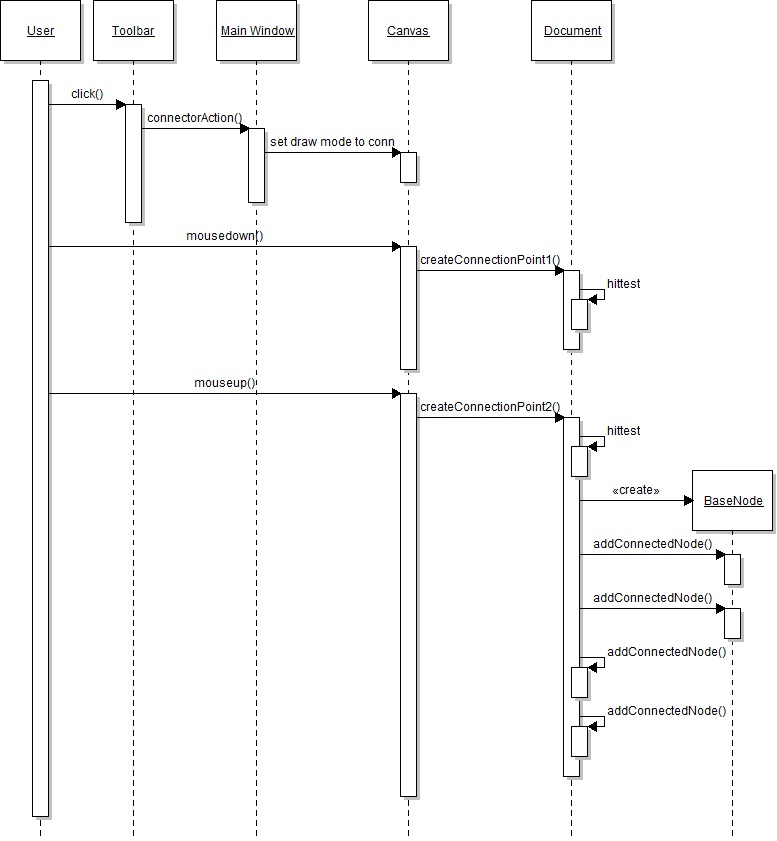
\includegraphics[width=5.0in]{IntNewConn.jpg}
\caption{Place New Connector}
\end{figure}

\clearpage




% 
% FEATURE: EDIT CONNECTOR DESCRIPTION
%

\subsubsection{Detailed Design for Feature: Edit Connector Description}

\paragraph[\ Introduction/Purpose of this Feature]
{\ Introduction/Purpose of this Feature}
{
User may edit a connector{\textquoteright}s description.
}

\paragraph[Input for this Feature]{Input for this Feature}
{
The user right clicks on a connector and selects ``Properties'' from the context menu.
}

\paragraph{Output for this Feature}
{
A dialog is displayed from which the user may make changes to the connector{\textquoteright}s description. After making a change, the new description will replace the existing description.
}

\paragraph{Feature Process to Convert Input to Output}
{
User right-clicks on the canvas. Canvas class setsSelectedConnector() to Document, which performs a hittest to verify the connector at the coordinates of the click. Then Document setSelectedConnector to itself. \newline
Canvas displays the context menu. The User clicks ``Properties'' and Canvas sends a showPropertiesDialog signal to Document, which in turn creates a properties Dialog.\newline
The User then modifies the properties, and Dialog sends the new properties information to Document.
}

\paragraph{Design Constraints and Performance Requirements of this Feature}
{
The user may not be able to edit all properties of all connectors due to the differences in connector utilization in differing UML diagrams. \newline
The user may only edit properties of valid objects and connectors. No other properties in pUML may be modified.
}
\bigskip
\bigskip

\begin{figure}[h]
\centering
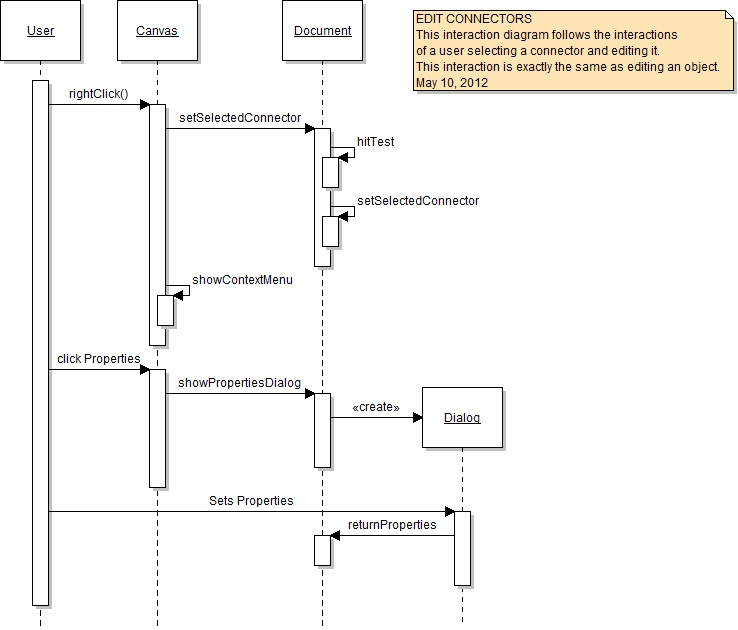
\includegraphics[width=6.0in]{IntEditConn.jpg}
\caption{Edit Connector Description}
\end{figure}

\clearpage



% 
% FEATURE: DELETE CONNECTOR
%

\subsubsection{Detailed Design for Feature: Delete Connector}

\paragraph[\ Introduction/Purpose of this Feature]
{\ Introduction/Purpose of this Feature}
{
The user deletes a connector from between two objects.
}

\paragraph[Input for this Feature]{Input for this Feature}
{
The user right-clicks on an connector, and selects ``Delete'' from the context menu.
}

\paragraph{Output for this Feature}
{
The connector no longer appears on the canvas.
}

\paragraph{Feature Process to Convert Input to Output}
{
User right clicks on an connector on the Canvas. The Canvas verifies through Document that a connector exists at the coordinates of the click, and sets the connector.  The Canvas displays a context menu.  The user selects the ``Delete'' option from the context menu.  Canvas tells Document to deleteSelectedConnector, and Document deletes the connector.
}

\paragraph{Design Constraints and Performance Requirements of this Feature}
{
N/A
}
\bigskip
\bigskip

\begin{figure}[h]
\centering
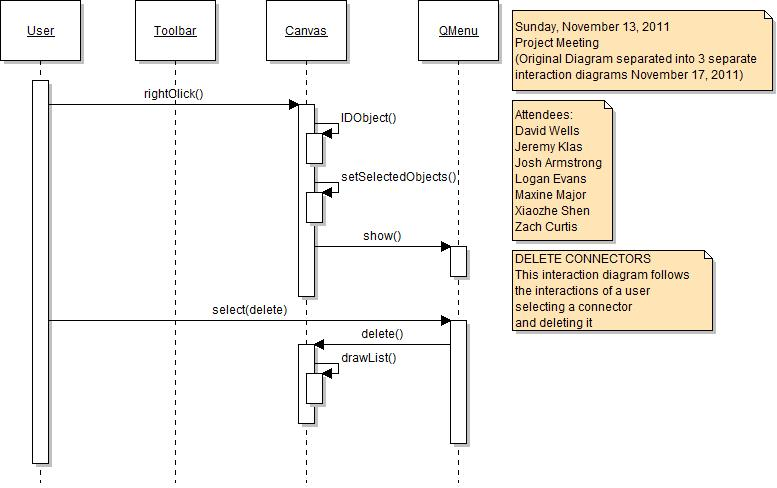
\includegraphics[width=6.0in]{IntDelConn.jpg}
\caption{Delete Connector}
\end{figure}

\clearpage

  





% **************************************
% SECTION 5: REQUIREMENTS TRACEABILITY *
% **************************************

\clearpage

\begin{landscape}

\section[REQUIREMENTS TRACEABILITY]
  {\bfseries REQUIREMENTS TRACEABILITY}
{\itshape }

\bigskip

\begin{flushleft}
\tablehead{}
\begin{supertabular}[c]{|
                        m{0.9in}|m{0.4in}|m{2.0in}|
                        m{0.4in}|m{0.5in}|m{1.0in}|
                        m{1.0in}|m{1.0in}|c|
                       }
\hline
 
  \centering \bfseries Feature Name &
  \centering \bfseries Req No. &
  \centering \bfseries Requirement Description &
  \centering \bfseries Priority &
  \centering \bfseries SSDD &
  \centering \bfseries Test Case(s) & 
  \centering \bfseries Alpha Release &
  \centering \bfseries Beta Release &
  \bfseries Final Test
\\\hline
  
  Install
  & \centering 2.2.1
  & pUML software installs successfully
  & \centering M 
  & N/A
  & testinstall
  & PASS
  & PASS
  & PASS
\\\hline

  Launch
  & \centering 2.2.1
  & pUML software launches successfully
  & \centering M 
  & N/A
  & testlaunch
  & PASS
  & PASS
  & PASS
\\\hline

  Exit
  & \centering 2.2.1
  & pUML Exit options 
  & \centering M 
  & 4.3.3
  & testsave *\newline
    testsaveas *
  & FAIL \newline
    FAIL 
  & PASS \newline
    PASS
  & PASS \newline
    PASS
\\\hline

  Main Window
  & \centering 2.2.2
  & All main window features 
  & \centering M 
  & *N/A
  & testmainwindow 
  & PASS
  & PASS
  & ~ 
\\\hline

  Objects
  & \centering 2.2.3
  & Object properties and functionality
  & \centering M 
  & 4.3.7 \newline
    4.3.8 \newline
    4.3.9 \newline
    4.3.10 
  & testobjects
  & PASS
  & PASS
  & ~ 
\\\hline

  Connectors
  & \centering 2.2.4
  & Connector properties and functionality
  & \centering M 
  & 4.3.11 \newline
    4.3.12 \newline
    4.3.13
  & testconnectors\newline 
    testselfconnector
  & FAIL \newline
    PASS
  & PASS \newline
    PASS
  & ~ \newline
    PASS
\\\hline

  Open
  & \centering 2.2.5
  & Load a pUML file into pUML 
  & \centering M 
  & 4.3.2
  & testsave *\newline
    testsaveas *
  & FAIL \newline
    FAIL 
  & PASS \newline
    PASS
  & ~ \newline
    ~
\\\hline

  Save/Save As
  & \centering 2.2.6
  & Save a diagram 
  & \centering M 
  & 4.3.4 \newline
    4.3.5 
  & testsave \newline 
    testsaveas
  & FAIL \newline
    PASS
  & PASS \newline
    PASS
  & ~ \newline
    ~
\\\hline

  Diagrams
  & \centering 2.2.7
  & Diagram type integrity 
  & \centering M 
  & 4.3.1
  & testsave *\newline 
    testsaveas *
  & FAIL \newline
    FAIL
  & PASS \newline
    PASS
  & ~ \newline
    ~
\\\hline

  Tabs
  & \centering 2.2.8
  & Tab functionality 
  & \centering M 
  & 4.3.6
  & testsave *\newline 
    testsaveas *
  & FAIL \newline
    FAIL
  & PASS \newline
    PASS
  & ~ \newline
    ~
\\\hline

\end{supertabular}
\end{flushleft}

{Priorities are: \textbf{M}andatory, \textbf{L}ow, \textbf{H}igh} \newline
{SSDD link is version and page number or function name.} \newline
{Test cases and results are file names and \textbf{P}ass/\textbf  {F}ail or \% passing.} \newline
{* asterisk indicates indirectly tested through another feature test case.}

\bigskip

\end{landscape}

\end{document}